\documentclass[a4paper,12pt]{article}
\usepackage{codeanatomy}
\usepackage{pgfplotstable}
\pgfplotsset{compat=1.18}
\usepackage{multicol}
\usepackage{booktabs}
\usepackage{amsmath}
\usepackage{graphicx}
\usepackage{float}
\usepackage{listings}
\usepackage{mathtools}
\usepackage[thinc]{esdiff}
\usepackage[T2A]{fontenc} 
\usepackage[utf8]{inputenc}
\usepackage{titlesec, titletoc} 
\usepackage{cmap} 
\usepackage[english,russian]{babel} 
\usepackage{caption}
\usepackage{xcolor} 
\usepackage{geometry}
    \geometry{left=30mm, right=20mm, top=20mm, bottom=20mm}

\titlespacing*{\section}{0pt}{2\baselineskip}{\baselineskip}
\titlespacing*{\subsection}{0pt}{2\baselineskip}{\baselineskip}
\titlespacing*{\subsubsection}{0pt}{2\baselineskip}{\baselineskip}


\definecolor{codegreen}{rgb}{0,0.6,0}
\definecolor{codegray}{rgb}{0.5,0.5,0.5}
\definecolor{codepurple}{rgb}{0.58,0,0.82}
\definecolor{backcolour}{rgb}{0.95,0.95,0.92}

\lstdefinestyle{mystyle}{
    backgroundcolor=\color{backcolour},   
    commentstyle=\color{codegreen},
    keywordstyle=\color{magenta},
    numberstyle=\tiny\color{codegray},
    stringstyle=\color{codepurple},
    basicstyle=\ttfamily\footnotesize,
    breakatwhitespace=false,         
    breaklines=true,                 
    captionpos=b,                    
    keepspaces=true,                 
    numbers=left,                    
    numbersep=5pt,                  
    showspaces=false,                
    showstringspaces=false,
    showtabs=false,                  
    tabsize=2
}

\lstset{style=mystyle}

\begin{document}

\noindent \textbf{ФИО:} Соловей Г.И. \hfill \textbf{Группа:} в5130904/30322

\section*{Работа №1. Ознакомление с основами векторной графики и получение
  навыков работы с базовыми функциями графического API и
  трехмерными графическими примитивами.}
\subsection* {Задание. Вариант 33}
Целью работы является ознакомление с основами векторной графики и получение
навыков работы с базовыми функциями графического API и трехмерными
графическими примитивами.
Требуется при помощи стандартных функций графической библиотеки
(OpenGL/WebGL/Vulkan) изобразить указанные объекты и произвести необходимые
преобразования.
\begin{enumerate}
    \item Изобразить каркасный чайник и поместить его в каркасный куб. Размеры и
          местоположение примитивов на экране задать самостоятельно.
    \item Повернуть чайник относительно начала координат на -30 градусов вокруг оси Х
    \item Изобразить конус и сферу, где вершина конуса является центром сферы.
    \item Переместить конус на dy=-30, масштабирование сферы с коэффициентом 1,5
\end{enumerate}

\subsection* {Выполнение задания}
Для выполнения всех лабораторных работ по предмету было решено использовать стандартную библиотеку OpenGL v.4.2 для C++ для рендеринга,
библиотеку GLFW для создания и управления окном, а также ImGui для для легкой отрисовки простых элементов интерфейса.
Библиотеку GLUT (FreeGLUT) было решено не использовать, так как она предоставляет функции устаревшего на данный
момент пайплайна графической отрисовки (fixed-function pipeline). В современном OpenGL большая часть рендеринга
возлагается на видеокарту посредством шейдеров, чтобы минимизировать использование процессора в пайплайне отрисовки.

Разработанная библиотека представляет собой упрощённый графический движок,
реализующий базовые компоненты современного графического приложения: управление окном,
камерой и процессом рендеринга.
Для управления зависимостями используется пакетный менеджер Conan 2.0.


Подробное описание и исходный код библиотеки см. в отчете к лабораторной работе 1.

Во второй работе библиотека используется для реализации более продвинутой системы материалов и освещения.

Основные этапы:
\begin {enumerate}
\item Инициализация приложения выполняется аналогично первой работе через класс Application, включая настройку окна и запуск графического цикла.
\item Расширение системы материалов: на основе базового класса Material реализованы пользовательские классы ColoredMaterial и TexturedMaterial, добавляющие поддержку освещения, цвета и текстур.
\item Работа с освещением: в материалах реализована передача параметров источника света (позиция и цвет) в шейдеры, что позволяет реализовать модели освещения (матовая, глянцевая).
\item Текстурирование: в TexturedMaterial добавлена загрузка и использование текстур, что расширяет визуальные возможности рендеринга.
\item Формирование сцены: используются как загружаемые модели (OBJMesh), так и примитивы (Cube, Sphere), к которым применяются различные типы материалов.
\item Интерактивное управление: через ImGui реализован интерфейс для изменения параметров камеры и источника света в реальном времени, а также переключения режима отрисовки.
\item Работа с прозрачностью: включено смешивание (glBlend), что позволяет корректно отображать полупрозрачные материалы.
\end {enumerate}

Таким образом, библиотека используется не только как каркас сцены, но и как основа для расширения системы рендеринга за счёт пользовательских материалов и освещения.
\subsection*{Вывод}
В ходе выполнения работы были изучены и реализованы принципы освещения и материалов в трёхмерной графике. Расширена базовая архитектура библиотеки путём создания собственных типов материалов с поддержкой цвета, освещения и текстур.

Были получены практические навыки работы с шейдерами, передачи параметров в GPU, а также реализации различных моделей освещения. Дополнительно освоены методы текстурирования и работа с прозрачностью.

В результате работы углублено понимание процесса рендеринга, а также приобретён опыт расширения графического движка и создания более реалистичных визуальных эффектов.
\newpage
\subsection*{Скриншоты результата работы}

\begin{figure}[H]
    \centering
    
\includegraphics[width=\textwidth]{images/image.png}
    \caption{Первичная сцена приложения}
\end{figure}
\begin{figure}[H]
    \centering
    
\includegraphics[width=\textwidth]{images/image.1.png}
    \caption{Сцена с увеличенной яркостью перемещенного света}
\end{figure}
\begin{figure}[H]
    \centering
    
\includegraphics[width=\textwidth]{images/image.2.png}
    \caption{Сцена с красным светом}
\end{figure}
\begin{figure}[H]
    \centering
    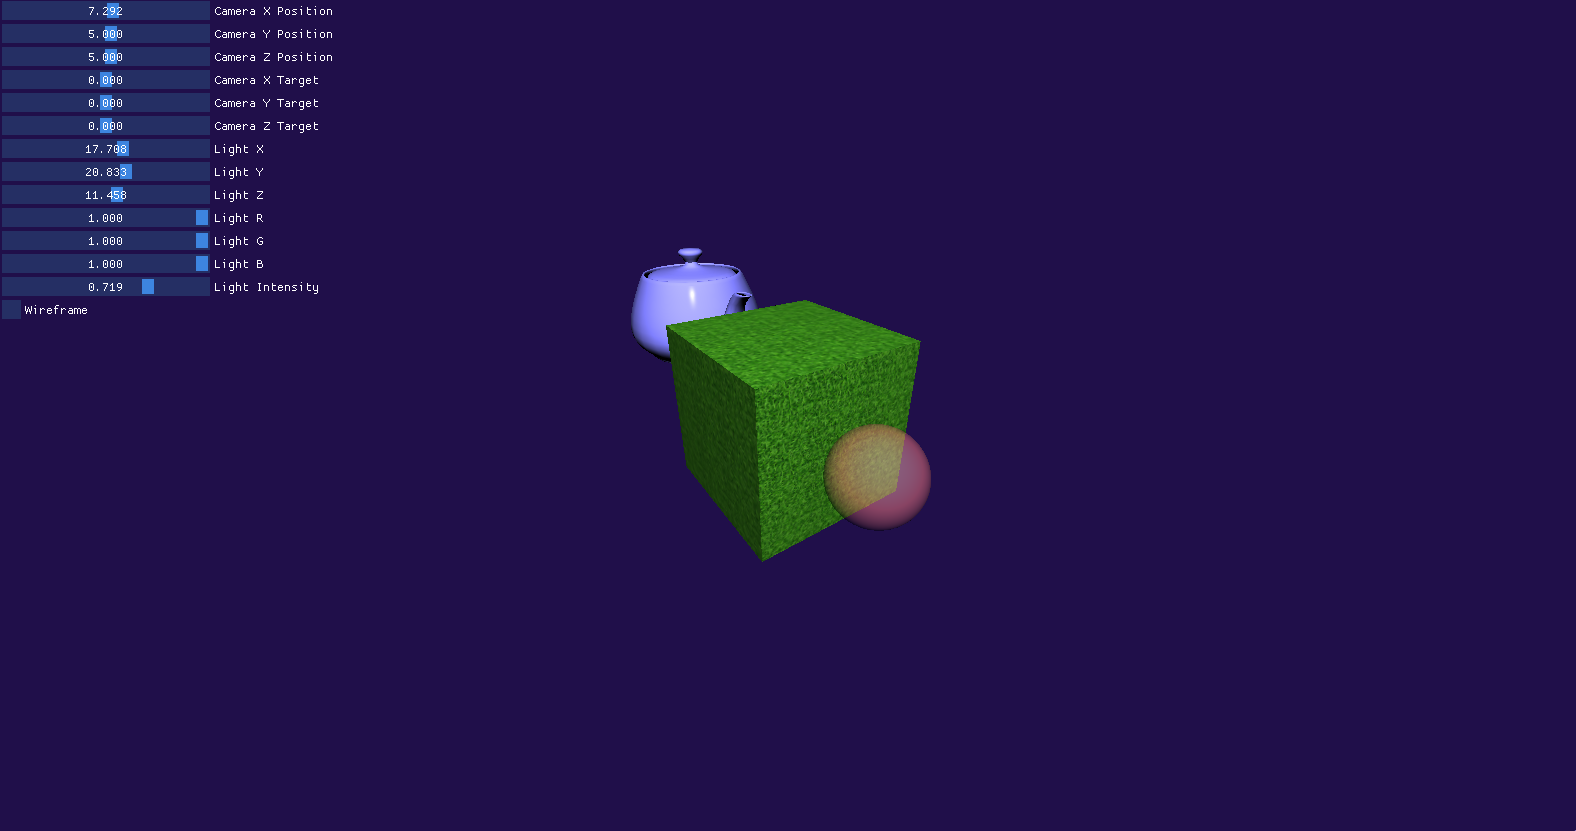
\includegraphics[width=\textwidth]{images/image.3.png}
    \caption{Сцена с демонстрацией полупрозрачности сферы}
\end{figure}


\subsection*{Исходный код работы}

\subsubsection*{textured\_material.cc}
\lstinputlisting{../src/c++/colored_material.cc}
\newpage

\subsubsection*{colored\_material.cc}
\lstinputlisting{../src/c++/colored_material.cc}
\newpage

\subsubsection*{main.cc}
\lstinputlisting{../src/c++/main.cc}
\newpage


\subsubsection*{Шейдер отполированной поверхности}
\lstinputlisting{../assets/shaders/glossy/frag.glsl}
\newpage

\subsubsection*{Шейдер матовой поверхности}
\lstinputlisting{../assets/shaders/matte/frag.glsl}
\newpage

\subsubsection*{Шейдер матовой текстурированной поверхности}
\lstinputlisting{../assets/shaders/textured/frag.glsl}
\newpage


\end{document}
